%
% File emnlp2015.tex
%
% Contact: daniele.pighin@gmail.com
%%
%% Based on the style files for ACL-2015, which were, in turn,
%% Based on the style files for ACL-2014, which were, in turn,
%% Based on the style files for ACL-2013, which were, in turn,
%% Based on the style files for ACL-2012, which were, in turn,
%% based on the style files for ACL-2011, which were, in turn, 
%% based on the style files for ACL-2010, which were, in turn, 
%% based on the style files for ACL-IJCNLP-2009, which were, in turn,
%% based on the style files for EACL-2009 and IJCNLP-2008...

%% Based on the style files for EACL 2006 by 
%%e.agirre@ehu.es or Sergi.Balari@uab.es
%% and that of ACL 08 by Joakim Nivre and Noah Smith

\documentclass[11pt,a4paper]{article}
\usepackage{acl2015}
\usepackage{times}
\usepackage{array}
\usepackage{url}
\usepackage{latexsym}
\usepackage{multirow}
\usepackage{graphicx}
\usepackage{epstopdf}

\usepackage[OPTIONS]{caption}

%\setlength\titlebox{5cm}

% You can expand the titlebox if you need extra space
% to show all the authors. Please do not make the titlebox
% smaller than 5cm (the original size); we will check this
% in the camera-ready version and ask you to change it back.

%% NOTE: not sure what sounds best. jot down whatever comes to mind here and decide later
\title{Dependency Parsing with LSTMs: An Empirical Evaluation}
%\title{Transition-Based LSTM Dependency Parser: An Empirical Evaluation}
% alternative titles:
% Best Practices for Dependency Parsing with LSTMs
% Empirical Evaluation and Best Practices for Dependency Parsing with LSTMs
% Empirical Evaluation and Best Practices for Transition-Based LSTM Dependency Parser
% Transition-Based LSTM Dependency Parser: An Empirical Evaluation

\author{Adhiguna Kuncoro$^{\spadesuit}$ ~ Yuichiro Sawai$^{\diamondsuit}$ ~ Kevin Duh$^{\heartsuit}$ ~ Yuji Matsumoto$^{\diamondsuit}$\\
$^{\spadesuit}$School of Computer Science, Carnegie Mellon University, Pittsburgh, PA, USA \\
$^{\diamondsuit}$Graduate School of Information Science, Nara Institute of Science and Technology, Japan \\
$^{\heartsuit}$HLTCOE, Johns Hopkins University, Baltimore, MD, USA\\
{\small \tt akuncoro@cs.cmu.edu, \{sawai.yuichiro.sn0,matsu  \}@is.naist.jp, kevinduh@cs.jhu.edu}
}

%\author{Adhiguna Kuncoro \\
%  \\\And
%  Yuichiro Sawai \\
%  %Graduate School of Information Science \\
%  %Nara Institute of Science and Technology \\
%  %{\tt \{adhiguna-k,sawai.yuichiro.sn0,kevinduh,matsu\}@is.naist.jp } %\\
%  \And
%  Kevin Duh \\\And
%  Yuji Matsumoto \\
%  }
  
\date{}

% for saving spaces around tables and figures
\setlength\textfloatsep{2truemm}
\setlength\intextsep{0pt}
\setlength\abovecaptionskip{1truemm}

\begin{document}
\maketitle
\begin{abstract}
We propose a transition-based dependency parser using Recurrent Neural Networks with Long Short-Term Memory (LSTM) units. This extends the feedforward neural network parser of \newcite{chenmanning14} and enables modelling of entire sequences of shift/reduce transition decisions. On the Google Web Treebank, our LSTM parser is competitive with the best feedforward parser on overall accuracy and notably achieves more than 3\% improvement for long-range dependencies, which has proved difficult for previous transition-based parsers due to error propagation and limited context information. Our findings additionally suggest that dropout regularisation on the embedding layer is crucial to improve the LSTM's generalisation.

%We propose a transition-based dependency parser using Recurrent Neural Networks with Long Short-Term Memory (LSTM) units. This extends the feedforward neural network parser of Chen and Manning (2014) and enables modelling of entire sequences of shift/reduce transition decisions. There are numerous design choices involved in LSTM models, each of which considerably affects parsing accuracy; our main contribution is an extensive empirical evaluation which suggests that the best practice involves a combination of high dropout rates and large numbers of hidden units. On the Google Web Treebank, our LSTM parser is competitive with the best feedforward parser on overall accuracy and achieves more than 3\% improvement for long-range dependencies.

\end{abstract}

\section{Introduction}

Two complementary approaches to transition-based dependency parsers have emerged recently. 
The {\em feature engineering} approach relies on hand-crafted feature templates to model interactions between sparse lexical features. While manually crafting these feature templates requires substantial expertise and extensive trial-and-error, this approach has led to state-of-the-art parsers in many languages \cite{BM06,ZN11}.

In contrast, the {\em neural network} approach enables automatic learning of feature combinations through  non-linear hidden layers and mitigates sparsity issues by sharing similar low-dimensional distributed  representations for related words \cite{Bet03}.
%As demonstrated by the recent work of Chen and Manning (2014), feedforward neural network parsers can also achieve state-of-the-art results. However, neural network models have their own challenges, as tuning the model architecture and hyperparameters is a similarly laborious process requiring substantial trial-and-error.\footnote{Which of the two approaches is more laborious is subject to debate--possibly an unproductive one.}

In this work, we explore new model architectures under the neural network approach. In particular, we address the issue that the feedforward architecture of the Chen and Manning parser performs training on each oracle configuration \textit{independently} of one another, disregarding the fact that the oracles for each training sentence represent a \textit{whole sequence} of intertwined decisions. Our proposed extension uses a Recurrent Neural Network (RNN) with Long Short-Term Memory (LSTM) units \cite{HS97}. At each time step of the transition system, the LSTM has theoretical access to the \textit{entire history} of past decisions (i.e. shift or reduce). LSTMs are naturally suited for modelling sequences and have shown promising results in e.g. machine translation \cite{Set14} and text-vision modelling \cite{Vet141}.

\par We particularly focus on the LSTM's performance in identifying \textit{long-range dependencies}. Such dependencies have proved difficult for most greedy transition-based parsers \cite{MN07}, including our feedforward baselines, that train on each oracle independently. This difficulty can be attributed to two main reasons: 1) most long-range dependencies are ambiguous, while the classifiers only have access to a limited context window, and 2) longer arcs are constructed after shorter arcs in transition-based parsing, thus increasing the chance of error propagation. In contrast, our LSTM has the key abilities of modelling  whole sequences of training oracles and memorise all past context information, both of which are likely beneficial for longer dependencies.

\par Despite the LSTM's theoretical advantages, in practice it is more prone to overfitting than the feedforward architecture, even with the same number of parameters. An additional contribution of this work is an empirical investigation that suggests that dropout \cite{Set142}, particularly when applied to the embedding layer, substantially improves the LSTM's generalisation ability regardless of hidden layer size. %Our parser is open-sourced: \url{http://to.be.released}.

%While the idea is conceptually simple, the implementation is not trivial. We document the important design choices in tuning the model architecture and hyperparameters. Interestingly, we discover that the combination of large hidden layers (which increases model capacity) and high dropout regularisation rates (which reduces the risk of overfitting) is best for LSTM parsing, while the lack of dropout leads to significantly poorer results. On the Google Web Treebank, our LSTM parser achieves competitive accuracy with the best feedforward model, and notably achieves more than 3\% improvement for long-range dependencies. 


\section{LSTM Parsing Model}

\begin{figure*}[t]
\setlength\belowcaptionskip{-1em}
\centering
\captionsetup{justification=centering}
  \begin{center}
    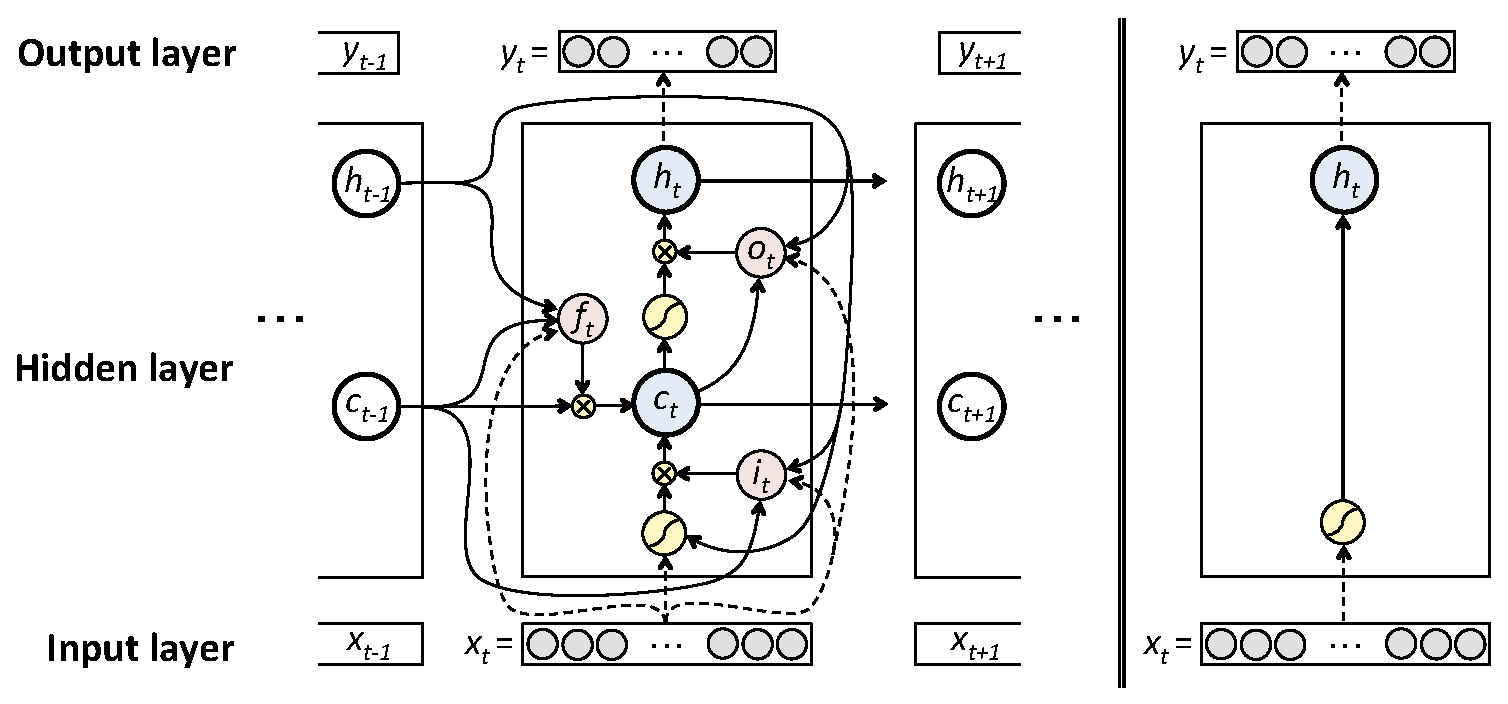
\includegraphics[width=0.85\linewidth]{images/fig_model.eps}
  \end{center}
  \setlength\abovecaptionskip{-.7truemm}
  \caption{Left: Our LSTM architecture. Right: Feedforward architecture in \newcite{chenmanning14}. Connections with dropout are denoted by dashed lines.}
\label{fig:model}
\end{figure*}

\subsection{Baseline Model}
Our model is an extension to \newcite{chenmanning14},
which uses a feedforward neural network to predict the next transition of an arc-standard system.
%In the arc-standard system, a configuration consists of a buffer $B$, a stack $S$, and a set of dependency arcs $A$.
%$B$ stores the input words, and the words are extracted from $B$ and pushed to $S$ as the dependency parsing proceeds and arcs are added to $A$.
In arc-standard, a configuration consists of a buffer $B$ (holding the input words), a stack $S$ (holding the partial parse trees), and a set of dependency arcs $A$.
The parse tree is built by successively making one of these transitions: 
\vspace{-.5em}
\begin{itemize}
\item SHIFT: move the next word on $B$ to $S$
\vspace{-.4em}
\item LEFT/RIGHT-ARC($L$): add left/right arc with label $L$ between top two words on $S$%, remove child
\end{itemize}
\vspace{-.5em}

%While feature engineering approaches like (Yamada and Matsumoto, 2003; Zhang and Nivre, 2011) use a classifier with sparse feature sets to decide which transition to take, the Chen and Manning model uses a feedforward neural network classifier with word, POS, and label embeddings as input features. In particular, their low-dimensional dense embedding features, which we term $x_t$, is a concatenation of embeddings from the top 3 words in $S$ and $B$, first and second left-/right-most children of the top two words on $S$, and the leftmost of leftmost / rightmost of rightmost children of the top two words on $S$. At each configuration at time $t$, the feedforward neural network first computes the hidden layer $h_t$ from the input $x_t$, then calculates the probability of each transition in the output vector $y_t:$\footnote{The dimension of $x_t$ is 2400 in experiments, and dimension of $y_t$ is $2|L|+1$, the number of possible transitions, with $|L|$ being number of dependency label types.}
The features $x_t$ is a concatenation of embeddings from the top 3 words in $S$ and $B$, first and second left-/right-most children of the top two words on $S$, and the leftmost of leftmost / rightmost of rightmost children of the top two words on $S$. At each configuration at time $t$, the neural network first computes the hidden layer $h_t$ from the input $x_t$ (applying a non-linear function $f$), then calculates the probability of each transition in the output vector $y_t:$\footnote{The dimension of $x_t$ is 2400 in experiments, and dimension of $y_t$ is $2|L|+1$, the number of possible transitions where $|L|$ = number of dependency label types.} %We omit bias terms in the equations for brevity.
\vspace{-1.0em}
\begin{eqnarray*}
  h_{t}\!\!\! &=& \!\!\! f (W_{xh} D(x_{t})) \\[-.2em]
  y_{t}\!\!\! &=& \!\!\! \mathrm{softmax} (W_{hy} D(h_{t}))
\end{eqnarray*}
$D(\cdot)$ is a dropout operator, which randomly sets elements to 0 with probability $p_{drop}$.
%$D(\cdot)$ is a dropout operator, which randomly sets elements to 0 with probability $p_{drop}$. In our notation, $W$ are matrix parameters to be learned and subscript like $W_{xh}$ indicate it connects $x$ (input) to $h$ (hidden layer). We ignore bias terms in the equations for brevity, though they are used in practice. 

\vspace{-.5em}
\subsection{Our LSTM Model}
%Our LSTM model uses the same $x_t$ features as (Chen and Manning, 2014), but importantly adds new inputs based on past information, e.g. previous hidden layer $h_{t-1}$. The addition of previous state leads to recurrence and thus theoretically enables modelling and training of the entire sequence of transitions. 
Our LSTM model (shown in Figure~\ref{fig:model}) uses the same $x_t$ features as \newcite{chenmanning14}, but importantly adds new inputs based on past information (such as $h_{t-1}$). The addition of previous state leads to recurrence and enables modelling and training of the entire sequence of transitions. 
%In practice, recurrence may cause the infamous "exploding gradient" and "vanishing gradient" (Bengio et al., 1994) problems, which lead to numerical difficulties in backpropagation training. 
%LSTM units provide an effective way to circumvent these numerical problems by introducing memory cells $c_t$ that could store information over long time intervals. What is stored in a memory cell $c_t$ is controlled by an input gate $i_t$, and whether the stored information is used in further computations is controlled by an output gate $o_t$. This allows information from the beginning of the sentence to influence transition actions at the end of the sentence. A forget gate $f_t$ is used to erase the information in the current memory cell. 

While recurrence may cause the ``vanishing gradient'' problem \cite{Bet94},
the LSTM architecture solves this by introducing memory cells $c_t$ that could store information over long time intervals and keep gradients from diminishing. Input gates $i_t$ control what is stored in a memory cell $c_t$, and output gates $o_t$ control whether the stored information is used in further computations. This allows information from the beginning of the sentence to influence transition actions at the end of the sentence. Forget gates $f_t$ are used to erase the information in the current memory cell. 

%The following equations describe our LSTM parser with peephole connections (Gers et al., 2002). Figure~\ref{fig:model} shows how each of the components connects. This LSTM unit setup follows the strategy set forth by~(Graves, 2013), while the recipe for successfully applying dropout to LSTM was investigated in Zaremba et al. (2014).
The following equations describe our LSTM model with peephole connections \cite{Get02}, as set forth by \newcite{G13}, and apply dropout similar to \newcite{Zet14}.
\vspace{-.6em}
\begin{eqnarray*}
  i_{t}\!\!\! &=& \!\!\! \sigma (W_{xi} D(x_{t}) + W_{ci} c_{t-1} + W_{hi} h_{t-1}) \\[-.25em]
  f_{t}\!\!\! &=& \!\!\! \sigma (W_{xf} D(x_{t}) + W_{cf} c_{t-1} + W_{hf} h_{t-1}) \\[-.25em]
  c_{t}\!\!\! &=& \!\!\! f_{t} c_{t-1}\! + \!i_{t} \ tanh (W_{xc} D(x_{t})\! + \!W_{hc} h_{t-1}\!) \\[-.25em]
  o_{t}\!\!\! &=& \!\!\! \sigma (W_{xo} D(x_{t}) + W_{co} c_{t} + W_{ho} h_{t-1}) \\[-.25em]
  h_{t}\!\!\! &=& \!\!\! o_{t} \ \tanh(c_{t}) \\[-.25em]
  y_{t}\!\!\! &=& \!\!\! \mathrm{softmax}(W_{hy} D(h_{t}))
\end{eqnarray*}

\vspace{-.6em}
%Crucially, the difference between the LSTM parser and feedforward parser is that the LSTM not only uses input $x_t$ in its predictions for $y_t$, but also exploits values in the previous memory cell $c_{t-1}$ and hidden layer $h_{t-1}$. Note that the gates $i_t$, $f_t$, and $o_t$ are bounded between $[0,1]$ due to the sigmoid $\sigma$, so their multiplication with other parts of the network modulates which information is passed through, e.g. $f_t$ and $i_t$ determine how much of the current memory $c_t$ depends on previous memory $c_{t-1}$, or current input $x_t$ plus previous hidden layer $h_{t-1}$. The gates have their own parameters (e.g. $W_{xi}$) and are learned jointly via backpropagation. 
Crucially, the LSTM not only uses input $x_t$ in its predictions for $y_t$, but also exploits values in the previous memory cell $c_{t-1}$ and hidden layer $h_{t-1}$ through the gates $i_t$, $f_t$, and $o_t$. The values of these gates are bounded between $[0,1]$ due to the sigmoid  $\sigma$, so multiplication with other components modulates what information is passed through. 

Given training sentences ${\{s_{i}\}}_{i=1}^{m}$ with gold parse trees,
our training data is a set of sequences of configurations $c_{it}$ and oracle transition actions $a_{it}$ at each time $t$ for each sentence $s_{i}$.
We maximise the log-likelihood of the oracle transition actions $a_{it}$ given by Equation (\ref{eq:ll}),
where $\theta$ is the set of parameters including word, POS, and label embeddings,
and $y_{t}(a)$ is the probability that the parser takes transition action $a$ at time $t$.
\vspace{-1em}
\begin{equation}
  L(\theta) = \sum_{i=1}^{m} \sum_{t} \log y_{t}(a_{it})
  - \frac{\lambda}{2} ||\theta||^2
  \label{eq:ll}
\end{equation}

\vspace{-1em}
We optimise by gradient backpropagation through time (BPTT) for each sentence $s_{i}$, feeding the parser with gold sequence of configurations $\{c_{it}\}_{t=1}^{|s_{i}|}$. 
When the parser reaches the final configuration, the gradients are backpropagated
from each prediction ${y_{it}}$ at time $t$ down to time $1$.
\section{Experiment}
\subsection{Experimental Settings} \label{exp_settings_large}
We conducted the experiments on the Google Web Treebank \cite{PM12}, consisting of the WSJ portion of the OntoNotes corpus and five additional web domains, with 48 dependency types. The models were trained only on the training set of the WSJ corpus, while the parameters were optimised using the WSJ dev set (i.e. no tuning using any of the web domains' dev set).

%We mapped all tokens to lowercase and converted numbers to a '0' token. We used the pre-trained embedding of Collobert et al. (2011) to initialise the word vectors (embedding size=50, coverage=87.7\%), while %POS-tag and label embeddings, along with the non-pre-trained words, 
%all other embeddings were initialised randomly between (-0.01, 0.01). All weight connections were initialised with the same mechanism as Glorot and Bengio (2010). %We trained on \textit{all} words of the training data, while unknown words in the dev and test set were assigned a single 'UNK' embedding \footnote{Since we train on all training words, the vector embedding for 'UNK' is not learnt during training}. 

As baselines, we re-implemented the Chen and Manning parser with the same setting, including results from both the feedforward model with Tanh activation function (same activation as the LSTM) and its better-performing Cubic counterpart. %All models were implemented in Python and Theano \cite{Bet10,Bet12}.
Training was done for a maximum of 400 epochs, stopped early if no better dev UAS was found after 30 consecutive epochs.\footnote{The LSTM was trained with the Adadelta optimiser \cite{Z12}, using a decay rate of 0.95 and $\epsilon=10^{-6}$. The embeddings were similarly initialised as the feedforward baselines, while the weight connections were initialised using the same mechanism as \newcite{GB10}.
We used automatic POS tags from the Stanford bi-directional tagger \cite{Tet03}, with tagging accuracies of 97\% for the WSJ and 87-92\% for the web domains.} 


%The feedforward baselines were trained using all the same hyper-parameters and Adagrad (Duchi et al., 2011) optimiser as Chen and Manning (2014), with the addition that we applied an input dropout rate of 0.05 on the embedding layer. Our best LSTM model has 150 hidden units, with a dropout rate of 0.6 applied on both the input-hidden and hidden-output connections (but not on the recurrent ones). 
%The LSTM was trained with the Adadelta optimiser \cite{Z12}, using a decay rate of 0.95 and $\epsilon=10^{-6}$. The embeddings were similarly initialised as the feedforward baselines, while the weight connections were initialised using the same mechanism as \newcite{GB10}. %For the LSTM model, we put sentences of the same length in the same batch, with a maximum batch size of 40 sentences. The LSTM model has about 1.6 millon parameters, compared to 500,000 for the feedforward baselines. 
%Training was done for a maximum of 400 epochs, stopped early if no better dev UAS was found after 30 consecutive epochs. %Training the feedforward and LSTM models took around 8 and 48 hours on an NVIDIA GTX680 GPU device, respectively, while both models similarly parsed 150 sentences per second using the GPU without pre-computation. 


\subsection{Main Result and Analysis}
\begin{figure*}[t]
\centering
\begin{minipage}{\columnwidth}
  \centering
  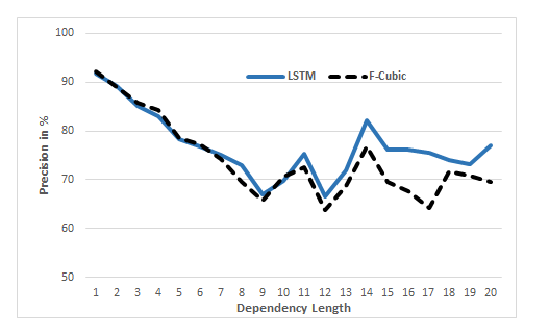
\includegraphics[width=.9\columnwidth]{images/precision.eps}
  \caption{Precision by Dependency Length}
  \label{fig:precision}
\end{minipage}
\begin{minipage}{.95\columnwidth}
  \centering
  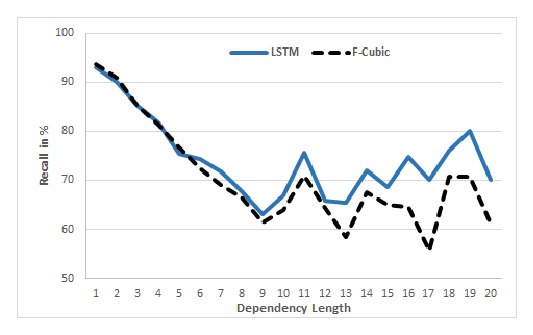
\includegraphics[width=.9\columnwidth]{images/recall.eps}
  \caption{Recall by Dependency Length}
  \label{fig:recall}
\end{minipage}
\end{figure*}
The LAS result on the Google Web Treebank is summarised on Table \ref{full_result_table}, where F-T and F-C represent the feedforward baselines with Tanh and Cubic activations, respectively.
Our LSTM model outperforms the feedforward baseline with the same Tanh activation function (87.5 vs 86.4 on WSJ Test), while achieving competitive accuracy with the Cubic baseline. 

We furthermore investigate the models' performance on long-range dependencies, reporting the result in terms of labelled precision and recall breakdown by dependency lengths on the WSJ test set in Table \ref{tab_long_range}. This result is also plotted in Figures \ref{fig:precision} and \ref{fig:recall}. 
Despite the models' similar overall accuracy, our LSTM model outperforms the Cubic baseline by more than 3\% in both precision and recall for dependency lengths greater than 7, and that the LSTM's performance degrades more slowly as dependency length increases.
%\footnote{Long-range dependencies only comprise 10\% of overall arcs, leading to similar overall accuracy}. 

%Since we did not tune on the web domains' dev set, we only show the test results of the web domains, using the "eval.pl" script for all final evaluation.

\begin{table}[t]
\centering
\begin{tabular}{|c|c|c|c|}
\hline
{\bf WSJ} & {\bf F - T} & {\bf F - C} & {\bf LSTM} \\ \hline
Dev             & 86.0        & 87.2        & {\bf 87.8} \\ \hline
Test            & 86.4        & {\bf 87.5}  & {\bf 87.5} \\ \hline \hline
{\bf Web Test}       & {\bf F - T} & {\bf F - C} & {\bf LSTM} \\ \hline
Answers         & 74.1        & {\bf 74.9}  & 74.6       \\ \hline
Emails          & 74.6        & {\bf 75.6}  & 74.4       \\ \hline
Newsgroups      & 79.3        & 79.9        & {\bf 80.2} \\ \hline
Reviews         & 76.5        & {\bf 77.2}  & 77.0       \\ \hline
Weblogs         & 80.7        & 81.1        & {\bf 81.2} \\ \hline
%{\bf Web Avg}   & 77.0        & {\bf 77.7}  & 77.5       \\ \hline
\end{tabular}
\caption{Google Web Treebank LAS Result}
\label{full_result_table}
\end{table}


%We additionally investigate the model's performance in identifying long-range dependencies. Such dependencies have proved difficult for most greedy transition-based parsers (McDonald and Nivre, 2007), including our feedforward baselines, that train on each oracle independently. This difficulty can be attributed to two main reasons: 1) most long-range dependencies are ambiguous, while the classifiers only have access to a limited context window, and 2) longer arcs are constructed after shorter arcs in transition-based parsing, thus increasing the chance of error propagation. In contrast, our LSTM model has two key advantages of modelling \textit{whole sequences} of training oracles, along with the theoretical ability to memorise all past context information, both of which are beneficial for longer dependencies.

\begin{table}[t]
\centering
\begin{tabular}{|c|c|c|c|c|}
\hline
{\bf \begin{tabular}[c]{@{}c@{}}Dep.\\ Length\end{tabular}} & \multicolumn{1}{l|}{} & F - T & F - C      & LSTM       \\ \hline
\multirow{2}{*}{1}                                          & Precision             & 91.4  & {\bf 92.2} & 91.7       \\ \cline{2-5} 
                                                            & Recall                & 93.1  & {\bf 93.6} & 93.0       \\ \hline
\multirow{2}{*}{2}                                          & Precision             & 87.9  & 88.9       & {\bf 89.3} \\ \cline{2-5} 
                                                            & Recall                & 90.3  & {\bf 91.0} & 90.1       \\ \hline
\multirow{2}{*}{3-6}                                        & Precision             & 81.7  & {\bf 83.4} & 82.6       \\ \cline{2-5} 
                                                            & Recall                & 79.2  & 81.3       & {\bf 81.4} \\ \hline
\multirow{2}{*}{7-49}                                       & Precision             & 68.1  & 70.3       & {\bf 73.5} \\ \cline{2-5} 
                                                            & Recall                & 62.6  & 65.6       & {\bf 69.5} \\ \hline
\end{tabular}
\caption{Long-range Arcs Precision \& Recall}
\label{tab_long_range}
\end{table}




\subsection{Regularisation Experiments}\label{hyperparameters}

We discover that regularisation is important for the LSTM parser, more so than feedforward architectures. Table \ref{table:with_without_dropout} compares the relative improvement due to dropout for feedforward vs. LSTM by constraining both models to have the same number of 500,000 parameters, corresponding to 50 hidden units for LSTM.
Observe that LSTM becomes competitive only with dropout. 

%Lastly, we investigated the impact of dropout on the performance of both the LSTM model and the Cubic baseline on the WSJ Test UAS. For the models without dropout, we trained the Cubic baseline with all the same hyper-parameters, while we reduced the number of hidden units of the non-dropout LSTM to 50 so that both models had a similar number of 500,000 parameters \footnote{Without dropout, larger LSTM models overfit and performed worse, constraining the size of our network}. The result is presented in Figure \ref{fig:with_without_dropout}. 

\begin{table}[h]
\centering
\begin{tabular}{|c|c|c|c|}
\hline
{\bf } & no dropout & with dropout & {\bf $\Delta$} \\ \hline
F-Cubic    & 89.1        & 89.5        & {\bf 0.4} \\ \hline
LSTM       & 87.4        & 89.5  & {\bf 2.1} \\ \hline
\end{tabular}
\caption{\label{table:with_without_dropout} Effect of Dropout on UAS Accuracy}
\end{table}


%\begin{figure}[h]
%\centering
%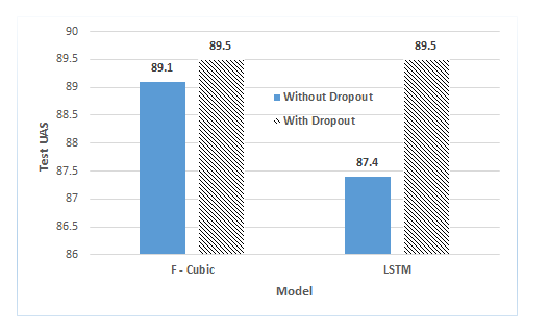
\includegraphics[scale=.95]{images/With_without_dropout.eps}
%\caption{Effect of Dropout on Accuracy}
%\label{fig:with_without_dropout}
%\end{figure}
%Despite the models' similar number of parameters, dropout significantly increased the LSTM model's accuracy, but not on Cubic baseline's. This result suggests that the LSTM model crucially requires regularisation to generalise well, which we investigate further in subsection \ref{hyperparameters}.

%Based on the previous finding, we empirically investigate various regularisation settings for the LSTM model and the correlation with hidden layer size. %We leave the analysis of other variations, such as optimisation method and LSTM architectures (e.g. peephole connections), to future work.

%To investigate what kind of dropout is beneficial,  we conducted further experiments on a subset of the training data (the first 80,000 tokens of the WSJ training set). We used the same experimental settings as in Subsection \ref{exp_settings_large} and evaluate UAS on the full WSJ dev and test set.
%except that training was done for a maximum of 500 epochs and stopped early if no better dev accuracy was found after 50 consecutive epochs. 
%\footnote{the UAS is calculated using the parser's internal evaluation, which might differ with the eval.pl script result}

To investigate what kind of dropout is beneficial,  we conducted further experiments on a subset of the training data (the first 80,000 tokens of the WSJ training set).\footnote{We used the same experimental settings as in Subsection \ref{exp_settings_large} and evaluate UAS on the full WSJ dev and test set, with hidden layer size fixed at 60.}
The results of dropout and L-2 regularisation are in Table \ref{tab_regul}, along with the epoch where the best dev UAS is found. E-H and H-O indicate dropout between the embedding-hidden and hidden-output connections, respectively. %For L-2, we performed a grid search in the log-linear space for L-2 coefficients between $10^{-3}$ and $10^{-8}$. For dropout, we experimented with three dropout rates: 0.2, 0.4, and 0.6, and apply each rate on three alternatives: on the embedding-hidden (E-H) connections, on the hidden-output (H-O) connections, and on both the embedding-hidden and hidden-output (E-H + H-O) connections. .

\begin{table}[t]
\centering
%\captionsetup{justification=centering}
\begin{tabular}{|c|c|c|c|c|}
\hline
\multicolumn{2}{|c|}{{\bf Reg Settings}} & {\bf Dev } & {\bf Test } & {\bf Epoch} \\ \hline \hline
\multicolumn{2}{|c|}{{\bf L2 $\lambda$}}    &               &                &             \\ \hline
\multicolumn{2}{|c|}{0}                  & 80.2         & 80.0           & 42          \\ \hline
\multicolumn{2}{|c|}{$10^{-8}$}                  & 80.7          & 80.8          & 25          \\ \hline
\multicolumn{2}{|c|}{$10^{-7}$}                  & 79.9          & 80.3           & 43          \\ \hline
\multicolumn{2}{|c|}{$10^{-6}$}                  & 79.8          & 80.1           & 43         \\ \hline
\multicolumn{2}{|c|}{$10^{-5}$}                  & 80.5          & 80.4          & 46          \\ \hline
\multicolumn{2}{|c|}{$10^{-4}$}                  & {\underline{83.4}}          & {\underline{82.9}}           & 206          \\ \hline
\multicolumn{2}{|c|}{$10^{-3}$}                  & 81.6          & 81.6           & 159          \\ \hline \hline
\multicolumn{2}{|c|}{\bf Dropout $p_{drop}$}  &               &                &             \\ \hline
\multirow{3}{*}{E-H}      & 0.2          & 84.4          & 84.3          & 97          \\ \cline{2-5} 
                          & 0.4          & 85.8          & {\underline{85.7}}           & 257          \\ \cline{2-5} 
                          & 0.6          & {\underline{\bf 86.2}}         & 85.5           & 273          \\ \hline
\multirow{3}{*}{H-O}      & 0.2          & 81.8          & 81.6          & 52          \\ \cline{2-5} 
                          & 0.4          & {\underline{82.3}}          & {\underline{82.1}}          & 93          \\ \cline{2-5} 
                          & 0.6          & 81.9          & 81.7          & 69          \\ \hline
\multirow{3}{*}{Both}  & 0.2          & 85.4          & 85.0          & 122          \\ \cline{2-5} 
                          & 0.4          & {\underline{86.1}}         & {\underline{\bf 85.9}}           & 315          \\ \cline{2-5} 
                          & 0.6          & 85.3          & 85.3           & 500          \\ \hline
\end{tabular}
\caption{UAS Accuracy of Various Regularisation}
\label{tab_regul}
\end{table}

While dropout generally results in slower convergence, the technique outperforms L-2 and significantly improves the model's accuracy by more than 6\%. Most importantly, we found input dropout to be more crucial than hidden-output dropout and achieves the same accuracy as dropout on both input and hidden layers, suggesting that our model can achieve good accuracy with input dropout alone. %\footnote{In contrast, hidden layer dropout is much more important for the feedforward model, and high input dropout rates hurt the feedforward model's performance}. 
We found dropout rates between 0.4 and 0.6 to be effective.
Further, we found that dropout generally improves LSTMs regardless of model size. Figure \ref{fig:dropout_hidden} shows how dropout of 0.5 on E-H and E-O layers improve results for various hidden layer sizes. 

\begin{figure}[t]
\centering
  \centering
  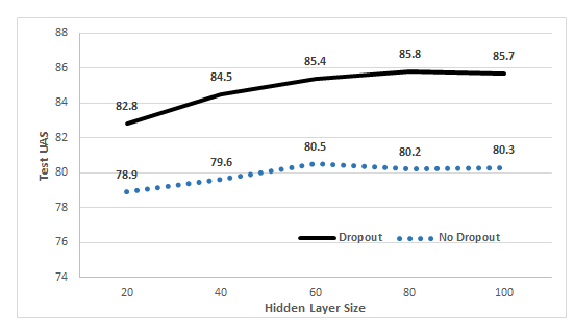
\includegraphics[width=.9\columnwidth]{images/dropout_hidden.eps}
  \caption{UAS Accuracy vs Hidden Layer Size}
\label{fig:dropout_hidden}
\end{figure}
%To investigate the correlation between dropout and hidden layer size, we applied a fixed dropout rate of 0.5 on both the embedding-hidden and hidden-output connections and experimented with hidden layer sizes from 20 to 100, in increments of 20. We compared the result with the models without dropout and summarised the test UAS result on Figure \ref{fig:dropout_hidden}. Importantly, dropout resulted in a sizable improvement even for small hidden layer sizes that are less prone to overfitting. This result indicates that dropout greatly improves generalisation ability and should be used regardless of model size. 




\section{Conclusions and Related Work}

We present a transition-based dependency parser using recurrent LSTM units. The motivation is to exploit the entire history of shift/reduce transitions when making predictions. This LSTM parser is competitive with the best feedforward neural network parser \cite{chenmanning14} on overall LAS, and notably improves the accuracy of long-range dependencies. We also show the importance of dropout, particularly on the embedding layer, in improving the model's accuracy.% and release the parser code to facilitate further investigations. 

{\bf Related work:} %There were several previous works that used RNNs for parsing. 
\newcite{Vet142} used LSTMs for sequence-to-sequence constituency parsing that makes no prior assumption of the parsing problem.
\newcite{S13} presented an RNN compositional model for dependency parsing, similar to the RNN constituency parser of \newcite{Set13}. 
Recently, the transition-based parser of \newcite{Det15} used stack LSTM architectures and represented the parser's internal stack and buffer contents with real-valued embedding.
In contrast, we present a simple LSTM parser that can still model whole training sequences and memorise all past states, which are beneficial for longer arcs. 

%Fonseca et al. (2015) used convolutional neural network to score edges in graph-based parsing, while the transition-based parser of Dyer et al. (2015) used stack LSTM architectures and represented the parser's internal stack and buffer contents with real-valued embedding.


%The previous work of Bansal et al. (2014) integrated word embeddings as additional features in existing transition-based parsers, although they did not use a neural network parsing model.

%In contrast, we present a simple, single layer LSTM parsing architecture that extends the previous work of \newcite{chenmanning14}. Despite its simplicity, our model still has a key advantage of modelling whole training sequences and potential to memorise all past states, which are beneficial for longer arcs. %The previous work of Greff et al. (2015) has analysed the effects of various LSTM hyper-parameters on three tasks that include speech recognition, although to the extent of our knowledge no such analysis has been done for LSTM dependency parsers.

%{\bf Future work:} There are a number of interesting directions for future work. The first possibility is to use a deep LSTM model, as such models have achieved state-of-the-art accuracy in many tasks such as speech recognition (Graves et al., 2013) and machine translation (Luong et al., 2014). 
%One may also represent the parser's internal states with real-valued vectors instead of relying on a fixed horizon of context window. 
%Another potential direction is to use beam search for training and testing, which substantially increased accuracy for the feature engineering approaches (Zhang and Clark, 2011).





\section*{Acknowledgments}

We thank Graham Neubig and Hiroyuki Shindo for the useful feedback and comments.  



% include your own bib file like this:
\nocite{*}
\newpage
\bibliographystyle{acl}
\bibliography{acl2015}




\end{document}
